\section{\texorpdfstring{$*$}{*}同调群的可计算性}
\sourcepage{63--64}
我们已计算过球面、环面和 Klein 瓶等熟悉空间的同调群。现在要问：一般情况下，同调群是否确实能够计算？对于有限复形，答案是肯定的。本节给出进行这种计算的明确算法。

首先证明一个基本定理，给出有限生成自由阿贝尔群之间同态的一种“标准形”，其证明是构造性的。第一个推论是前面陈述的关于自由阿贝尔群子群的定理 1.5.2；第二个推论是自由链复形的标准基定理；第三个推论给出所需的有限复形同调群计算算法。

先证明两个你可能已熟悉的引理。

\entry{引理}{1.12.1}设 $A$ 为秩为 $n$ 的自由阿贝尔群。若 $B$ 为 $A$ 的子群，则 $B$ 为秩 $r\leq n$ 的自由阿贝尔群。

\noindent\textbf{证明：}不妨设 $B$ 为 $n$ 重直积 $\Z^n=\Z\times\cdots\times\Z$ 的子群。如下构造 $B$ 的基。

以 $\pi_i:\Z^n\to\Z$ 表示第 $i$ 坐标投影。对于每个 $m\leq n$，定义
\[
B_m=B\cap(\Z^m\times0).
\]
也就是说，$B_m$ 由所有对 $i>m$ 满足 $\pi_i(x)=0$ 的 $x\in B$ 组成。特别地，$B_n=B$。同态 $\pi_m:B_m\to\Z$ 的像是 $\Z$ 的子群。若此子群平凡，令 $x_m=0$；否则选取 $x_m\in B_m$，使 $\pi_m(x_m)$ 生成该子群。断言：$\{x_1,\ldots,x_n\}$ 中的非零元素构成 $B$ 的一组基。

先证明，对每个 $m$，$x_1,\ldots,x_m$ 生成 $B_m$，从而全部 $x_i$ 生成 $B$。对 $m$ 归纳。$x_1$ 生成 $B_1$ 是显然的：若 $d=\pi_1(x_1)$，则 $x_1=(d,0,\ldots,0)$，而 $B_1$ 恰由其所有整数倍组成。即使 $x_1=0,d=0$，仍如此。

设 $x_1,\ldots,x_{m-1}$ 生成 $B_{m-1}$，取 $x\in B_m$。对某个整数 $k$，有 $\pi_m(x)=k\pi_m(x_m)$，所以 $\pi_m(x-kx_m)=0$，即 $x-kx_m\in B_{m-1}$。由归纳假设，
\[
x-kx_m=k_1x_1+\cdots+k_{m-1}x_{m-1},
\]
故 $x_1,\ldots,x_m$ 生成 $B_m$。

其次，对每个 $m$，证明 $\{x_1,\ldots,x_m\}$ 中非零元素的独立性。仍用归纳，$m=1$ 时平凡。设 $m-1$ 时成立。若
\[
\lambda_1x_1+\cdots+\lambda_mx_m=0,
\]
只需证明对每个 $x_i\ne0$ 都有 $\lambda_i=0$。作用 $\pi_m$ 得 $\lambda_m\pi_m(x_m)=0$。因此要么 $\lambda_m=0$，要么 $x_m=0$：若 $\lambda_m\ne0$，则 $\pi_m(x_m)=0$，从而子群 $\pi_m(B_m)$ 平凡，依定义 $x_m=0$。所以
\[
\lambda_m=0\quad\text{若 }x_m\ne0,\qquad
\lambda_1x_1+\cdots+\lambda_{m-1}x_{m-1}=0.
\]
再用归纳假设，即得对 $i<m$，只要 $x_i\ne0$ 就有 $\lambda_i=0$。\hfill$\square$

为后文所用，将此结果推广到任意自由阿贝尔群。

\entry{引理}{1.12.2}若 $A$ 为自由阿贝尔群，则其任意子群 $B$ 都自由。

\noindent\textbf{证明：}上面对有限情形的证明可推广到 $A$ 有无限基的情形。利用良序定理，它等价于选择公理，用具有最大元素的良序集 $J$ 给 $A$ 的基编号。

不妨设 $A$ 等于若干 $\Z$ 的副本的直和，即 $\Z^J$ 中所有只有有限多个非零坐标的元组 $(n_\alpha)_{\alpha\in J}$ 组成的子群。之后的方法与前面一样；由于这个过程可能不熟悉，给出细节。

设 $B$ 为 $A$ 的子群。对于 $\beta\in J$，令 $B_\beta$ 由所有当 $\alpha>\beta$ 时满足 $\pi_\alpha(x)=0$ 的 $x\in B$ 组成。考察 $\Z$ 的子群 $\pi_\beta(B_\beta)$：若其平凡，令 $x_\beta=0$；否则选取 $x_\beta\in B_\beta$，使 $\pi_\beta(x_\beta)$ 生成此子群。

\sourcepage{65}
先证明 $\{x_\alpha:\alpha\leq\beta\}$ 生成 $B_\beta$。若 $\beta$ 是 $J$ 的最小元素，这显然成立。一般地，用超限归纳。给定 $x\in B_\beta$，对某个整数 $k$，有 $\pi_\beta(x)=k\pi_\beta(x_\beta)$，故 $\pi_\beta(x-kx_\beta)=0$。考虑使 $\pi_\alpha(x-kx_\beta)\ne0$ 的所有指标 $\alpha$。若没有，则 $x=kx_\beta$，证明结束。否则，由 $x,x_\beta\in B_\beta$ 知，这些指标都小于 $\beta$；且它们只有有限多个，所以存在最大值 $\gamma<\beta$。于是 $x-kx_\beta\in B_\gamma$，由归纳假设，它可写成各 $x_\alpha$（$\alpha\leq\gamma$）的线性组合。

再证明 $\{x_\alpha:\alpha\leq\beta\}$ 中非零元素的独立性。$\beta$ 最小时平凡。一般地，设
\[
\lambda_{\alpha_1}x_{\alpha_1}+\cdots+\lambda_{\alpha_k}x_{\alpha_k}
+\lambda_\beta x_\beta=0,\qquad \alpha_i<\beta.
\]
作用 $\pi_\beta$ 得 $\lambda_\beta\pi_\beta(x_\beta)=0$。与前面一样，要么 $\lambda_\beta=0$，要么 $x_\beta=0$。所以当 $x_\beta\ne0$ 时，$\lambda_\beta=0$，并有
\[
\lambda_{\alpha_1}x_{\alpha_1}+\cdots+\lambda_{\alpha_k}x_{\alpha_k}=0.
\]
归纳假设说明，只要 $x_{\alpha_i}\ne0$，就有 $\lambda_{\alpha_i}=0$。\hfill$\square$

现在证明基本定理，先作一个定义。

\entry{定义}{1.12.3}设自由阿贝尔群 $G,G'$ 分别有基 $a_1,\ldots,a_n$ 与 $a'_1,\ldots,a'_m$。若 $f:G\to G'$ 为同态，则对于唯一确定的整数 $\lambda_{ij}$，有
\[
f(a_j)=\sum_{i=1}^m\lambda_{ij}a'_i.
\]
矩阵 $(\lambda_{ij})$ 称为 $f$ 关于给定基的\textbf{矩阵}。

\entry{定理}{1.12.4}设 $G,G'$ 分别为秩 $n,m$ 的自由阿贝尔群，$f:G\to G'$ 为同态。存在它们的基，使 $f$ 关于这些基的矩阵具有形式
\[
B=\begin{pmatrix}
\operatorname{diag}(b_1,\ldots,b_\ell)&0\\0&0
\end{pmatrix},\qquad b_i\geq1,\quad b_1\mid b_2\mid\cdots\mid b_\ell.
\]
此矩阵由 $f$ 唯一确定，尽管相应的基并不唯一。称它为 $f$ 的矩阵的\textbf{标准形}（normal form）。

\sourcepage{66--67}
\noindent\textbf{证明：}先任意为 $G,G'$ 选择基，令 $A$ 为 $f$ 关于它们的矩阵。下面给出修改基的过程，使矩阵化为定理的标准形，从而证明定理。

\entry{定义}{1.12.5}整数矩阵 $A$ 的\textbf{初等行变换}为：
\begin{enumerate}[label=(\arabic*)]
\item 交换第 $i$ 行与第 $k$ 行。
\item 第 $i$ 行乘以 $-1$。
\item 用“第 $i$ 行 $+q$ 倍第 $k$ 行”替换第 $i$ 行，其中 $q$ 为整数，$k\ne i$。
\end{enumerate}
每种变换都对应 $G'$ 中的基变换：第一种交换 $a'_i,a'_k$；第二种将 $a'_i$ 换为 $-a'_i$；第三种将 $a'_k$ 换为 $a'_k-qa'_i$，容易验证。还有三种类似的\textbf{初等列变换}，对应 $G$ 中的基变换。

下面说明如何用这六种初等变换，把任意整数矩阵 $A$ 化为所需标准形。设 $A$ 不是零矩阵，否则平凡。开始介绍算法之前，先注意：若整数 $c$ 整除 $A$ 的每个元素，且 $B$ 由 $A$ 经过任意一种初等变换得到，则 $c$ 也整除 $B$ 的每个元素。

\subsection*{化简算法}
算法从给定的非零整数矩阵 $A=(a_{ij})$ 出发，使用初等变换产生定理 1.12.4 的化简形式。

\entry{定义}{1.12.6}对非零整数矩阵 $A=(a_{ij})$，令 $\alpha(A)$ 为各数 $|a_{ij}|$ 中最小的非零值。若 $|a_{ij}|=\alpha(A)$，则称 $a_{ij}$ 为 $A$ 的一个\textbf{最小元素}。

\entry{引理}{1.12.7}设 $A$ 为非零整数矩阵。$\alpha(A)$ 不能整除 $A$ 的某个元素，当且仅当可以对 $A$ 施行初等变换，使 $\alpha$ 的值减小。

\noindent\textbf{证明：}设最小元素 $a_{ij}$ 不能整除 $A$ 的某个元素。若它不能整除同列的元素 $a_{kj}$，用 Euclid 除法引理写成
\[
a_{kj}=qa_{ij}+r,\qquad0<|r|<|a_{ij}|.
\]
这里不必限制符号，$q,r$ 均可正可负。将第 $k$ 行换为“第 $k$ 行减去 $q$ 倍第 $i$ 行”，\translatornote{原文将行操作印为“第 $i$ 行减去 $q$ 倍第 $k$ 行”，但紧接着计算的是 $a_{kj}-qa_{ij}=r$，应为此处的操作。}则新矩阵第 $k$ 行第 $j$ 列的元素为 $r$，所以新矩阵的 $\alpha$ 至多为 $|r|$，小于 $\alpha(A)$。若 $a_{ij}$ 不能整除同行的某个元素，也类似。

最后，设 $a_{ij}$ 整除其所在行、列的每个元素，但不能整除某个 $a_{st}$，其中 $s\ne i,t\ne j$。考察四个位置
\[
\begin{matrix}a_{ij}&\cdots&a_{it}\\\vdots&&\vdots\\a_{sj}&\cdots&a_{st}\end{matrix}.
\]
由于 $a_{ij}\mid a_{sj}$，可用初等行变换使这些位置成为
\[
\begin{matrix}a_{ij}&\cdots&a_{it}\\\vdots&&\vdots\\0&\cdots&a_{st}+\ell a_{it}\end{matrix}.
\]
再将第 $i$ 行换为第 $i$ 行与第 $s$ 行之和，得到
\[
\begin{matrix}a_{ij}&\cdots&a_{st}+(\ell+1)a_{it}\\\vdots&&\vdots\\0&\cdots&a_{st}+\ell a_{it}\end{matrix}.
\]
因为 $a_{ij}\mid a_{it}$，它不能整除 $a_{st}+(\ell+1)a_{it}$，于是回到不能整除同行某元素的情形。

反方向，若 $\alpha(A)$ 整除 $A$ 的每个元素，则初等变换得到的任何矩阵 $B$ 仍非零，且 $\alpha(A)$ 仍整除其每个元素。选择任意非零元素 $b_{ij}$，则 $|b_{ij}|\geq\alpha(A)$。\hfill$\square$

\sourcepage{68}
\noindent\textbf{算法的主要步骤。}设给定分块矩阵
\[
\begin{pmatrix}\operatorname{diag}(b_1,\ldots,b_k)&0\\0&A\end{pmatrix},\tag{$*$}
\]
满足：
\begin{enumerate}[label=(\arabic*)]
\item 正整数集 $\{b_1,\ldots,b_k\}$ 可以为空，且 $b_1\mid\cdots\mid b_k$。
\item $A$ 为非零整数矩阵，$b_k$ 整除其所有元素。
\end{enumerate}
对 $A$ 作初等变换，相当于对大矩阵 $(*)$ 的相应行、列作同样变换。

令 $A_0=A$。由引理 1.12.7，若 $\alpha(A_0)$ 不整除 $A_0$ 的每个元素，则可施行初等变换，得到满足 $\alpha(A_1)<\alpha(A_0)$ 的矩阵 $A_1$。重复这个过程，不超过 $\alpha(A_0)$ 次，就得到 $\alpha(A_r)$ 整除每个元素的矩阵 $A_r$。继续变换它，但为方便仍记作 $A_r$。

把一个最小元素移至左上角，并使其为正。因为它整除同行同列的所有元素，可以用初等变换把同行同列的其他元素都化为零。此过程结束后，左上角元素仍整除矩阵的每个元素，特别是整除删去第一行、第一列后得到的子矩阵 $A'$ 的所有元素。以 $b_{k+1}$ 表示此左上角元素。

于是，经过初等变换，$(*)$ 化为
\[
\begin{pmatrix}
\operatorname{diag}(b_1,\ldots,b_k)&0&0\\
0&b_{k+1}&0\\0&0&A'
\end{pmatrix},
\]
其中 $b_i\geq1$，$b_1\mid\cdots\mid b_k\mid b_{k+1}$，$b_{k+1}$ 整除 $A'$ 的每个元素，而且 $A'$ 比 $A$ 少一行、一列。

\noindent\textbf{终止条件。}若 $A'$ 全为零或为空，就得到所需标准形；否则重复主要步骤。

\noindent\textbf{定理 1.12.4 证明的完成。}由第 1.5 节习题 4，各数 $b_1,\ldots,b_\ell$ 由同态 $f$ 唯一确定。事实上，非零元素个数 $\ell$ 正是自由阿贝尔群 $f(G)\subset G'$ 的秩，而大于 $1$ 的那些 $b_i$ 正是商群 $G'/f(G)$ 的挠系数 $t_1,\ldots,t_k$。\translatornote{原文称 $G'/f(G)$ 为“挠群”，它一般还可有自由部分；所需的是其挠系数。}\hfill$\square$

\sourcepage{69}
\subsection*{化简算法的应用}
现在证明第 1.5 节陈述的自由阿贝尔群子群基本定理。

\noindent\textbf{定理 1.5.2 的证明：}给定秩为 $n$ 的自由阿贝尔群 $F$，由引理 1.12.1，任意子群 $R$ 都自由，秩 $r\leq n$。考察包含同态 $j:R\to F$，为 $R$ 选择基 $a_1,\ldots,a_r$，为 $F$ 选择基 $e_1,\ldots,e_n$，使 $j$ 的矩阵具有定理 1.12.4 的标准形。由于 $j$ 为单同态，这个标准形没有零列。所以对 $i=1,\ldots,r$，$j(a_i)=b_i e_i$，其中 $b_i\geq1$ 且 $b_1\mid\cdots\mid b_r$。因为 $j(a_i)=a_i$，故 $b_1e_1,\ldots,b_re_r$ 为 $R$ 的一组基。\hfill$\square$

现在引入链复形，并证明自由链复形的标准基定理。

\entry{定义}{1.12.8}\textbf{链复形}（chain complex）$\mathcal C$ 是由整数编号的一列阿贝尔群及同态
\[
\cdots\longrightarrow C_{p+1}\xrightarrow{\partial_{p+1}}C_p
\xrightarrow{\partial_p}C_{p-1}\longrightarrow\cdots,
\]
满足对所有 $p$，有 $\partial_p\circ\partial_{p+1}=0$。定义其第 $p$ 同调群为
\[
H_p(\mathcal C)=\ker\partial_p/\operatorname{im}\partial_{p+1}.
\]
若此群有限生成，其 Betti 数和挠系数称为 $\mathcal C$ 的 $p$ 维 Betti 数和挠系数。

\entry{定理}{1.12.9（自由链复形的标准基）}设 $\{C_p,\partial_p\}$ 为链复形，每个 $C_p$ 都为有限秩自由群。对于每个 $p$，存在 $C_p$ 的子群 $U_p,V_p,W_p$，使
\[
C_p=U_p\oplus V_p\oplus W_p,
\]
其中 $\partial_p(U_p)\subset W_{p-1}$，$\partial_p(V_p)=0$，$\partial_p(W_p)=0$。此外，存在 $U_p$ 与 $W_{p-1}$ 的基，使 $\partial_p:U_p\to W_{p-1}$ 的矩阵为
\[
\operatorname{diag}(b_1,\ldots,b_\ell),\qquad
b_i\geq1,\quad b_1\mid\cdots\mid b_\ell.
\]

\sourcepage{70--71}
\noindent\textbf{证明：第一步。}令 $Z_p=\ker\partial_p$，$B_p=\operatorname{im}\partial_{p+1}$。令 $W_p$ 为所有某个非零整数倍属于 $B_p$ 的元素 $c_p\in C_p$ 构成的集合。这是 $C_p$ 的子群，称为\textbf{弱边界群}（group of weak boundaries）。有
\[
B_p\subset W_p\subset Z_p\subset C_p.
\]
第二个包含关系成立，是因为链群无挠：由 $mc_p=\partial_{p+1}d_{p+1}$ 得 $m\partial_pc_p=0$，从而 $\partial_pc_p=0$。\translatornote{原文此处说 $C_p$ 无挠；这一步实际使用的是 $C_{p-1}$ 无挠，而定理的假设保证了这一点。}

考察自然投影 $Z_p\to H_p(\mathcal C)\to H_p(\mathcal C)/T_p(\mathcal C)$，其中 $T_p$ 为挠子群。其核为 $W_p$，所以 $Z_p/W_p\cong H_p/T_p$。后者有限生成且无挠，故自由。若 $c_1+W_p,\ldots,c_k+W_p$ 为 $Z_p/W_p$ 的基，$d_1,\ldots,d_\ell$ 为 $W_p$ 的基，则容易验证 $c_1,\ldots,c_k,d_1,\ldots,d_\ell$ 为 $Z_p$ 的基。因此 $Z_p=V_p\oplus W_p$，其中 $V_p$ 以 $c_1,\ldots,c_k$ 为基。

\textbf{第二步。}选择 $C_p$ 的基 $e_1,\ldots,e_n$ 和 $C_{p-1}$ 的基 $e'_1,\ldots,e'_m$，使 $\partial_p$ 的矩阵为标准形：对 $i\leq\ell$，$\partial_pe_i=b_i e'_i$；对 $i>\ell$，$\partial_pe_i=0$，其中 $b_i\geq1$，$b_1\mid\cdots\mid b_\ell$。则：
\begin{enumerate}[label=(\arabic*)]
\item $e_{\ell+1},\ldots,e_n$ 为 $Z_p$ 的一组基。
\item $e'_1,\ldots,e'_\ell$ 为 $W_{p-1}$ 的一组基。
\item $b_1e'_1,\ldots,b_\ell e'_\ell$ 为 $B_{p-1}$ 的一组基。
\end{enumerate}
证明如下。一般的 $p$ 维链及其边界为
\[
c_p=\sum_{i=1}^n a_i e_i,\qquad
\partial_pc_p=\sum_{i=1}^\ell a_i b_i e'_i.
\]
因为 $b_i\ne0$，此链为闭链，当且仅当 $i=1,\ldots,\ell$ 时 $a_i=0$，这证明了 (1)。任何边界 $\partial_pc_p$ 都位于 $b_1e'_1,\ldots,b_\ell e'_\ell$ 生成的群中，而这些元素独立，证明了 (3)。最后证明 (2)：每个 $e'_i$（$i\leq\ell$）属于 $W_{p-1}$，因为 $b_i e'_i=\partial e_i$。反过来，若
\[
c_{p-1}=\sum_{i=1}^m d_i e'_i\in W_{p-1},
\]
则对于某个 $\lambda\ne0$，有
\[
\lambda c_{p-1}=\partial_pc_p=\sum_{i=1}^\ell a_i b_i e'_i.
\]
比较系数，对 $i>\ell$ 得 $\lambda d_i=0$，故 $d_i=0$。因此 $e'_1,\ldots,e'_\ell$ 为 $W_{p-1}$ 的基。\translatornote{原文在此最后一句将下标印作 $W_{-1}$。}

\textbf{第三步。}选择第二步的基，令 $U_p$ 由 $e_1,\ldots,e_\ell$ 张成，则 $C_p=U_p\oplus Z_p$。按第一步选取 $V_p$，使 $Z_p=V_p\oplus W_p$。于是得到所需分解，且 $\partial_p(V_p)=\partial_p(W_p)=0$。$U_p,W_{p-1}$ 的所需基由第二步得到。\hfill$\square$

注意，$W_p$ 与 $Z_p=V_p\oplus W_p$ 是 $C_p$ 中唯一确定的子群，而 $U_p,V_p$ 并不唯一。

\entry{定理}{1.12.10}有限复形 $K$ 的同调群可以有效计算。

\noindent\textbf{证明：}由前一定理，存在分解 $C_p(K)=U_p\oplus V_p\oplus W_p$，其中 $Z_p=V_p\oplus W_p$ 为闭链群，$W_p$ 为弱边界群。有
\[
H_p(K)=Z_p/B_p\cong V_p\oplus(W_p/B_p)
\cong(Z_p/W_p)\oplus(W_p/B_p).
\]
$Z_p/W_p$ 自由，$W_p/B_p$ 为挠群，所以计算 $H_p(K)$ 归结为计算这两个群。

固定地给 $K$ 的单形定向，为每个链群选择基。边界同态 $\partial_p:C_p(K)\to C_{p-1}(K)$ 关于这些基的矩阵元素均属于 $\{-1,0,1\}$。利用前述算法将它化为标准形。从上个证明第二步的结果可得：
\begin{enumerate}[label=(\arabic*)]
\item $Z_p$ 的秩等于零列的个数。
\item $W_{p-1}$ 的秩等于非零行的个数。
\item $W_{p-1}/B_{p-1}\cong\Z/b_1\oplus\cdots\oplus\Z/b_\ell$。
\end{enumerate}
\sourcepage{72--73}
因此，$\partial_p$ 的矩阵标准形给出 $K$ 的 $p-1$ 维挠系数，即其中大于 $1$ 的元素；它也给出 $Z_p$ 的秩。另一方面，$\partial_{p+1}$ 的标准形给出 $W_p$ 的秩。两个秩之差就是 $Z_p/W_p$ 的秩，即 $K$ 的 $p$ 维 Betti 数。\hfill$\square$

\subsection*{习题}
\begin{enumerate}
\item 证明：若只计算有限复形 $K$ 的 Betti 数，不需要上述化简算法，只需要一个求矩阵秩的算法。具体地，若 $A_p$ 是 $\partial_p:C_p(K)\to C_{p-1}(K)$ 关于某些基的矩阵，则
\[
\beta_p(K)=\operatorname{rank}C_p(K)-\operatorname{rank}A_p-\operatorname{rank}A_{p+1}.
\]
\item 计算图 1.12.1 所示商空间的同调群。［提示：先检查是否所有顶点都被等同。］
\begin{center}
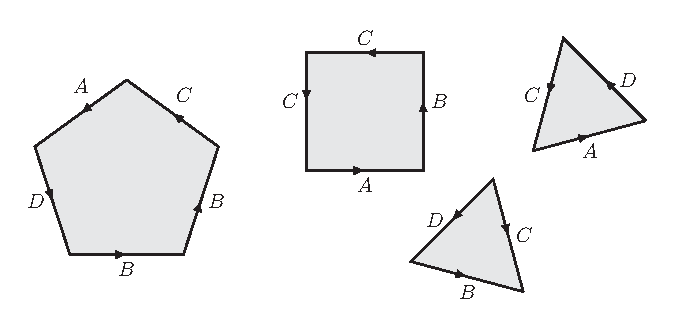
\includegraphics[width=117mm]{figures/1-12-1.pdf}\\图 1.12.1
\end{center}
\item 将下列矩阵化为标准形：
\[
\begin{pmatrix}2&6&4\\4&-7&4\\4&8&4\end{pmatrix}.
\]
\end{enumerate}
